\documentclass[a4paper,12pt]{article}
\usepackage[english]{babel}
\usepackage[utf8]{inputenc}

% Larger borders -- we do not want do waste paper, even if it is only paper on screen =)
\usepackage[top=2.5cm, bottom=2.5cm, left=2cm, right=2cm]{geometry}
% Remove auto indentation of paragraphs.
\setlength\parindent{0pt}

% Palatino font (nicer serif font: Times is for oldies)
\renewcommand*\rmdefault{ppl}

% Nested itemize list bullet style
\renewcommand{\labelitemi}{$\bullet$}
\renewcommand{\labelitemii}{$\circ$}
\renewcommand{\labelitemiii}{--}

% Math packages
\usepackage{mathtools}
\usepackage{amsmath}
\usepackage{amsfonts}
\usepackage{amssymb}

% Graphic packages
\usepackage{graphicx}
\usepackage{float}
\usepackage{adjustbox}
\usepackage{tikz}
\usepackage{forest,array}
\usetikzlibrary{shadows}

% Graphs styles
\forestset{
  giombatree/.style={
    for tree={
      grow = east,
      parent anchor=east,
      child anchor=west,
      edge={rounded corners=2mm},
      fill=violet!5,
      drop shadow,
      l sep=10mm,
      edge path={
        \noexpand\path [draw, \forestoption{edge}] (!u.parent anchor) -- +(5mm,0) -- (.child anchor)\forestoption{edge label};
      }
    }
  }
}
\forestset{
  qtree/.style={
    for tree={
      parent anchor=south,
      child anchor=north,
      align=center,
      edge={rounded corners=2mm},
      fill=violet!5,
      drop shadow,
      l sep=10mm,
    }
  }
}

% BAN logic macros
\newcommand{\believes}{\mid\!\equiv}
\newcommand{\sees}{\triangleleft}
\newcommand{\oncesaid}{\mid\!\sim}
\newcommand{\controls}{\Rightarrow}
\newcommand{\fresh}[1]{\#(#1)}
\newcommand{\combine}[2]{{\langle #1 \rangle}_{#2}}
\newcommand{\encrypt}[2]{{ \{ #1 \} }_{#2}}
\newcommand{\sharekey}[1]{\xleftrightarrow{#1}}
\newcommand{\pubkey}[1]{\xmapsto{#1}}
\newcommand{\secret}[1]{\xleftrightharpoons{#1}}

\newcommand{\projectname}{Cybersec.proj}

% Hides ugly links from the index
\usepackage[hidelinks]{hyperref}
% Landscape format pdf pagess
\usepackage{pdflscape}

\title{Cybersecurity Project}
\author{F. Barbarulo, G. B. Rolandi, Bruk T. Gurmesa}

\begin{document}
\maketitle
\tableofcontents

\clearpage

\section{Introduction}
\projectname{} is a client-server application which allows to download and upload files on a server in a secure manner.

\section{Application layer protocol}
Application layer manages its input/output data as continuos infinite stream of bytes.

Application sends and receives request commands and reply statuses, and generic streams of bytes (the body), whose meaning depends on the previous sent/received command/reply.

The protocol vaguely resembles HTTP.

A \texttt{parola} is defined as a pure ASCII sequence which can match the following regular expression \texttt{[A-Za-z0-9\textbackslash.\_]*}.
Different \texttt{parola}s can be separed by a whitespace.

Every command must be composed by one or more \texttt{parola}s.

\subsection{Request commands}
A request command is sent by the client to the server.

Generic structure of a request command is:
\begin{verbatim}
COMM filename\n
tag: value\n
\n
body
\end{verbatim}

Each line is terminated by a \texttt{LF} char, and each command is terminated by a \texttt{LF} char.
It is important to send the line feed char because server will not parse the command until two trailing \texttt{LF}s are received.

Note: a \texttt{LF} char is represented by a byte whose value is \texttt{0x0A}.
\\
A command is composed by the following parts:
\begin{itemize}
  \item \texttt{COMM} is a 4 char \texttt{parola} and represents the command to issue;
  \item \texttt{filename} is the name of a file on which issue the command.
  Filenames are composed by one \texttt{parola}.
  Depending on the specific command, a filename is mandatory or forbidden;
  \item \texttt{tag: value} is a pair of two \texttt{parola}s, composed by a \texttt{parola} immediately followed by a colon, a whitespace and another \texttt{parola}.
  First \texttt{parola} represents the tag for an additional parameter of current command, while second one representes the actual value for the parameter; depending on the specific command, one or more parameters may be mandatory or forbidden;
  \item \texttt{body} is a stream of bytes whose length must be specified in a command parameter; depending on the specific command, a body is mandatory or forbidden:
\end{itemize}

\subsection{Reply status}
A reply status is sent by the server to the client.

Generic structure of a reply status is:

\begin{verbatim}
DDD\n
tag: value
\n
body
\end{verbatim}

A reply status is composed by the following parts:
\begin{itemize}
  \item \texttt{DDD} a 3 ASCII digits number representing the state of the previous request command;
  \item \texttt{tag: value} is a pair to represent a parameter, with the same format of the request command parameter; depending on the specific command, one or more parameters may be mandatory or forbidden;
  \item \texttt{body} is a stream of bytes whose length must be specified in a reply status parameter; depending on the specific command the reply refers to, a body is mandatory or forbidden;
\end{itemize}

\subsection{Request commands list}

\paragraph{DELE}
\texttt{DELE filename}

Reply status:
\begin{itemize}
  \item \texttt{200}: ok
  \item \texttt{452}: bad file
\end{itemize}

\paragraph{LIST}
\texttt{LIST}

Request the server to send a list of available files

Reply status:
\begin{verbatim}
200\n
Size: listsize\n
\n
body
\end{verbatim}

\texttt{body} is a list of \texttt{parola}, each one representing the name of a file and each one separed by a newline.

\paragraph{QUIT}
\texttt{QUIT}

Close connection with the server.

Reply status:
\begin{itemize}
  \item \texttt{200}: ok
\end{itemize}

\paragraph{RETR}
\texttt{RETR filename}

Retrieve a file from the server.

Reply status:
\begin{itemize}
  \item success:
\begin{verbatim}
200\n
Size: filesize\n
\n
body
\end{verbatim}
  \item failure:\\
  \texttt{452}: bad file
\end{itemize}

\paragraph{STOR}
\begin{verbatim}
STOR filename
Size: filesize

body
\end{verbatim}

Store a file on the remote server, possibly overwriting an existing one.

\begin{itemize}
  \item \texttt{Size: filesize} is a parameter pair. \texttt{filesize} is the decimal ASCII representation of the file size in bytes;
  \item \texttt{body} is the actual content of the file;
\end{itemize}

Reply status:
\begin{itemize}
  \item \texttt{200}: ok
\end{itemize}

\subsection{Generic return values}
\begin{itemize}
  \item \texttt{500}: server error
  \item \texttt{501}: syntax error
  \item \texttt{502}: command not implemented
  \item \texttt{503}: bad sequence of commands
\end{itemize}

\section{Secure layer session protocol}
Every time that the application layer calls the secure layer with new data to send to the other party, a special secure layer packet is created; the receiver then expects to receive the same kind of packet, and extracts data from it to pass to the application level.

Receiver's side transparently checks these packet's validity, and then unfolds them and passes them to the application layer as a stream of bytes.

\begin{figure}[H]
\centering
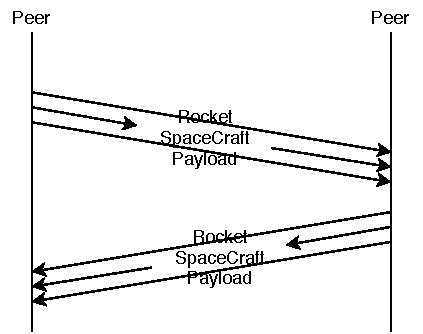
\includegraphics{img/secure-session-protocol.pdf}
\caption{Secure layer session protocol overview}
\end{figure}

\subsection{Secure packets}
Secure packets have two fixed length headers, called \texttt{Rocket} and \texttt{SpaceCraft}.
Every integer has network byte order endianess.

\subsection{Rocket}
First, \texttt{Rocket} is sent (or received).

\begin{verbatim}
struct Rocket {
  unsigned char hmac[HMAC_LEN],
  uint32_t length,
  uint32_t sequence_number
};
\end{verbatim}

where

\begin{itemize}
  \item \texttt{hmac} is used to authenticate Rocket's content;
  \item \texttt{length} is the size, in bytes, of the variable length payload and it is used to allocate data at receiver's endpoint;
  \item \texttt{sequence\_number} is used to protect against replay attacks;
\end{itemize}

After the \texttt{Rocket}'s content has been authenticated, its content is used to prepare the receiver's buffer.
Then, \texttt{Rocket} can be detached and control passes entirely to \texttt{spacecraft}.

\subsection{SpaceCraft}
A \texttt{SpaceCraft} always follows the \texttt{Rocket}.

\begin{verbatim}
struct SpaceCraft {
  unsigned char hmac[HMAC_LEN],
  uint32_t sequence_number
};
\end{verbatim}

where

\begin{itemize}
  \item \texttt{hmac[]} is used to authenticate SpaceCraft's content;
  \item \texttt{sequence\_number} is used to protect against replay attacks;
\end{itemize}

\subsection{Encrypted Payload}
Finally, the encrypted payload follows the \texttt{SpaceCraft}.

The encrypted payload can be of any length between $0$ and $2^{32}$ bytes, even if in our implementation it has a practical limitation of $4k$ bytes.

The payload is encrypted using AES128 in CFB mode, using a \emph{session key} and an \emph{initialization vector} that are exchanged during the initial handshake.

// TODO

\begin{itemize}
  \item \texttt{session_key}
  \item \texttt{iv}
\end{itemize}

\section{Key exchange protocol}
A 3 way handshake is needed in order to establish the secure session.

\begin{figure}[H]
\centering
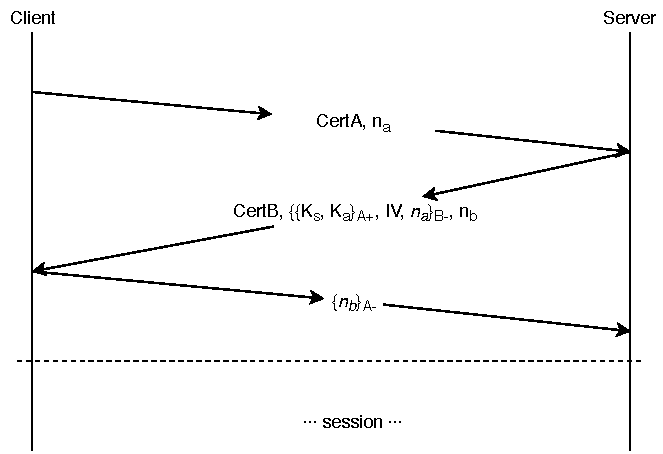
\includegraphics{img/key-exchange-protocol.pdf}
\caption{Key exchange protocol overview}
\end{figure}

\subsection{Objectives}

\[A \believes A \sharekey{k_s} B \]
%\[B \believes A \sharekey{k_s} B \]
\[A \believes \fresh{A \sharekey{k_s} B} \]

\subsection{Assumptions}

\paragraph{Keys}

\[A \believes \pubkey{CA^+} CA \]
\[B \believes \pubkey{CA^+} CA \]

\paragraph{Trust}

\[A \believes B \controls A \sharekey{k_s} B \]
\[A \believes B \controls \fresh{A \sharekey{k_s} B} \]
\[A \believes CA \controls (cert_A, cert_B) \]
\[B \believes CA \controls (cert_A, cert_B) \]

\paragraph{Freshness}

\[A \believes \fresh{R_A} \]
\[B \believes \fresh{R_B} \]
\[B \controls \fresh{A \sharekey{k_s} B} \]

\subsection{Proof}

\begin{align}
\frac{A \believes \pubkey{CA^+} CA, A \sees \encrypt{cert_B}{CA^-}}{A \believes CA \oncesaid cert_B} \tag*{postulate 1}
\end{align}

\begin{align}
\frac{A \believes CA \believes cert_B, A \believes CA \controls cert_B}{A \believes cert_B} \tag*{postulate 3}
\end{align}

$A \believes cert_B$ means that $A \believes \pubkey{B^+} B$, since $\pubkey{B+} B$ is part of $cert_B$

\begin{align}
\frac{A \believes \pubkey{B^+} B, A \sees \encrypt{payload_{M2}}{B^-}}{A \believes B \oncesaid payload_{M2}} \tag*{postulate 1}
\end{align}

\begin{align}
\frac{A \believes \fresh{payload_{M2}, A \believes B \oncesaid payload_{M2}}}{A \believes B \believes payload_{M2}} \tag*{postulate 2}
\end{align}

$\fresh{payload_{M2}}$ is due to the fact that it contains $R_A$, that is known to be fresh.

\begin{align}
\frac{A \believes B \believes payload_{M2}, A \believes B \controls payload_{M2}}{A \believes payload_{M2}} \tag*{postulate 3}
\end{align}

This means that $A \believes A \sharekey{k_s} B$
\end{document}
